\documentclass[11pt, a4paper]{article}
\usepackage[T1]{fontenc}
\usepackage[utf8]{inputenc}
\usepackage[polish]{babel}
\usepackage{amsmath}
\usepackage{amsfonts}
\usepackage{graphicx}
\usepackage{listings}
\usepackage{color}
\author{Kamil Kuczaj}
\date{\today}
\title{Sprawozdanie - Dynamiczna Alokacja Pamięci}


\begin{document}

\maketitle

\section{Wstęp}
Podanym zadaniem był pomiar czasu wykonywania alokacji pamięci dla tablicy dynamicznej elementów typu \textit{int}. Należało wykonać pomiary zapisu: $10^1$, $10^3$, $10^5$, $10^6$, $10^9$ danych oraz stworzyć specjalną klasę, która będzie zarządzać zapisem danych oraz alokacją pamięci. Poniżej listing pliku nagłówkowego klasy.

\lstset{
	language=C++,
    basicstyle=\ttfamily,
    keywordstyle=\color{blue}\ttfamily,
    stringstyle=\color{red}\ttfamily,
    commentstyle=\color{green}\ttfamily,
    morecomment=[l][\color{magenta}]{\#}
	caption=Descriptive Caption Text, 
  	basicstyle=\footnotesize, frame=tb,
    xleftmargin=.2\textwidth, xrightmargin=.2\textwidth
}
\begin{figure}[h]
	\begin{center}
		\begin{lstlisting}
class pojemnik  {
 private:
  int *elementy;
  unsigned long rozmiar;
  unsigned long indeks;

 public:
  pojemnik(int x=10);
  ~pojemnik();
  bool czy_pelne();
  void zapisz(int dana);  
  int zwieksz_rozmiar();  
  unsigned long zwroc_rozmiar();
  void wypisz(); // w celu debuggowania
};
		\end{lstlisting}
		\caption{Listing pliku \textit{pojemnik.h}}
	\end{center}
\end{figure}

\section{Specyfikacja komputera}

\begin{center}
	\begin{tabular}{| r | c |}
	\hline
	Wersja kompilatora \textit{g++} & 4.8.4 \\ \hline
	System & Ubuntu 14.04.4 \\ \hline
	Procesor	 & Intel Core i5 2510M 2.3 GHz \\ \hline
	Pamięć RAM & 8 GB DDR3 1600 MHz \\ \hline
	Rozmiar zmiennej \textit{int} & 4 bajty \\ \hline
	\end{tabular}
\end{center}


\section{Wybrane metody alokacji pamięci i wyniki}

\begin{enumerate}
	\item Zwiększanie rozmiaru tablicy o $1$ element
		\begin{center}
		\begin{tabular}{| p{5cm} | p{5cm} |}
			\hline
			Rozmiar & Ilość elementów \\ \hline
			$10$ & $1\ \mu s$ \\ \hline
			$1\ 000$ & $1,63\ ms$ \\ \hline
			$100\ 000$ & $18,483\ s $ \\ \hline
			$1\ 000\ 000$ & $2070,91\ s=~34,5 min$ \\ \hline
			$1\ 000\ 000\ 000$ & zbyt długo \\ \hline
     	\end{tabular}
     	%\includegraphics[scale=•]{•}
	\end{center}
	\item Zwiększanie rozmiaru tablicy o $100$ elementów
		\begin{center}
		\begin{tabular}{| p{5cm} | p{5cm} |}
			\hline
			Rozmiar & Ilość elementów \\ \hline
			$10$ & $1\ \mu s$ \\ \hline
 			$1\ 010$ & $33\ \mu s$ \\ \hline
			$100\ 010$ & $206,995\ ms$ \\ \hline
        		$1\ 000\ 010$ & $19,7127\ s$ \\ \hline
			$1\ 000\ 000\ 000$ & zbyt długo \\ \hline
	    \end{tabular}
	    %\includegraphics[scale=•]{•}	
	    \end{center}
	\item Zwiększanie rozmiaru tablicy o $10 000$ elementów
		\begin{center}
		\begin{tabular}{| p{5cm} | p{5cm} |}
			\hline
			Rozmiar & Ilość elementów \\ \hline
			$10$ & $1\ \mu s$ \\ \hline
          	$10\ 010$ & $14\ \mu s$ \\ \hline
 			$100\ 010$ & $3,097\ ms$ \\ \hline
        		$1\ 000\ 010$ & $227,339\ ms$ \\ \hline
			$1\ 000\ 000\ 000$ & zbyt długo \\ \hline
	    \end{tabular}
	    %\includegraphics[scale=•]{•}	
	    \end{center}
	\item Podwajanie rozmiaru tablicy
		\begin{center}
		\begin{tabular}{| p{5cm} | p{5cm} |}
			\hline
			Rozmiar & Ilość elementów \\ \hline
        		$10$ &  $2\ \mu s$ \\ \hline
	        $1\ 280$ & $25\ \mu s$ \\ \hline
	        $163\ 840$ & $2,381\ ms$ \\ \hline                                                            
    		    $1\ 310\ 720$ & $20,657\ ms$ \\ \hline
	    \end{tabular}
	    %\includegraphics[scale=•]{•}
	    \end{center}
	    Przy większych ilościach danych następował wyciek pamięci, gdyż potrzebna
	    była zbyt duża ilość pamięci danych:\\
	    $$1310720*2^{10}=1342177280\ (>10^9)$$
	    \[ \frac{1310720*2^{10}}{{2^{20}}}*4=5\ 120\ MB \]
	    Program więc potrzebował 5 GB pamięci podręcznej, czego mój system nie mógł
	    zapewnić.
	    
	\item Potrajanie rozmiaru tabliicy
		\begin{center}
		\begin{tabular}{| p{5cm} | p{5cm} |}
			\hline
			Rozmiar & Ilość elementów \\ \hline
			$10$ & $1\ \mu s$ \\ \hline
            $2\ 430$ & $17\ \mu s$ \\ \hline
         	$196\ 830$ & $1,375\ ms$ \\ \hline
        		$1\ 771\ 470$ & $15,127\ ms$ \\ \hline   
	    \end{tabular}
	    %\includegraphics[scale=•]{•}	
	    \end{center}
    	    Przy większych ilościach danych następował wyciek pamięci, gdyż potrzebna
	    była zbyt duża ilość pamięci danych tak jak w poprzednio wyjaśnionym przypadku.
	    
	\item Zwiększanie rozmiaru tablicy o $50\%$
		\begin{center}
		\begin{tabular}{| p{5cm} | p{5cm} |}
			\hline
			Rozmiar & Ilość elementów \\ \hline
			$10$ & $1\ \mu s$ \\ \hline
            $1\ 234$ & $29\ \mu s$ \\ \hline 
         	$106\ 710$ & $2,017\ ms$ \\ \hline
        		$1\ 215\ 487$ & $20,354\ ms$ \\ \hline  
	    \end{tabular}
	    %\includegraphics[scale=•]{•}	
	    \end{center}  
   	    Przy większych ilościach danych następował wyciek pamięci, gdyż potrzebna
	    była zbyt duża ilość pamięci danych tak jak w poprzednio wyjaśnionym przypadku.
	    
\end{enumerate}

\section{Wnioski}
\ \ \ \ Choć najbardziej optymalną metodą zwiększania rozmiaru tablicy jest jej podwajanie, to przy bardzo dużych danych może się skończyć brakiem pamięci fizycznej wynikającej z ograniczeń sprzętowych (zbyt mała ilość pamięci RAM komputera). To samo tyczy się potrajania rozmiaru tablicy oraz zwiększania jej rozmiaru o 50\%. Niemniej jednak są to bardzo wydajne metody.

Żadna z metod dodawania elementów, nawet w ilościach takich jak $10\ 000$ nie dorównują wspomnianym powyżej metodom. Poniżej zamieściłem wykres ilustrujący szybkość zapisu trzech najwydajniejszych metod.
\begin{figure}[h]
\begin{center}
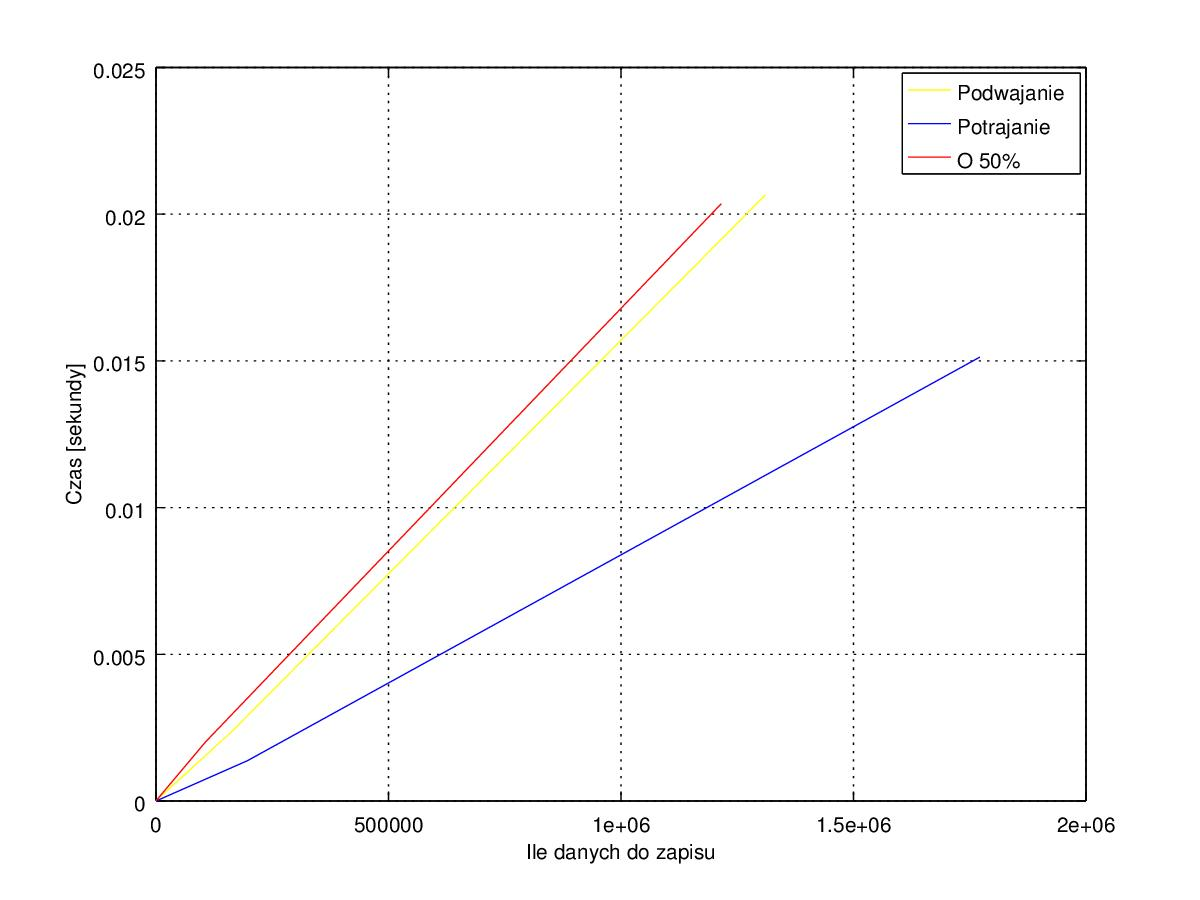
\includegraphics[width=1.2\textwidth]{wykres.jpg}
\end{center}
\caption{Wyraźnie widać, że najlepszą metodą w eksperymencie okazało się potrajanie rozmiaru tablicy}
\end{figure}


\end{document}